% Provenance (never printed): old seconde/premiere S material on the ocean
% (the ocean as a layered fluid, its heat, upwelling and productive waters);
% see sources/book2/PROVENANCE.md. All profiles are WOA23 columns, all
% densities the EOS-80 one-atmosphere equation, computed in
% figdata/grade-10/ocean_profiles.py.
\chapter{Samudra yang Berlapis}\label{ch:g10:layered-ocean}

Pada suatu hari musim panas kamu berenang dari pantai ke air yang hangat dan
nyaman. Lalu kamu membiarkan kakimu menjuntai ke bawah --- dan telapak kakimu
mendapati air yang tiba-tiba dingin, beberapa meter di bawah permukaan. Laut
tidak tercampur dari atas sampai ke bawah: laut tersusun atas lapisan-lapisan,
yang hangat dan ringan di atas, yang dingin dan rapat di bawah. Di samudra
terbuka, pelapisan yang sama mencapai kedalaman berkilometer-kilometer, dan
pelapisan itulah yang menentukan di mana laut menjadi gurun dan di mana laut
penuh kehidupan. Bab ini membahas samudra menurut kedalamannya: bagaimana
samudra diukur, bagaimana suhu dan salinitasnya berubah ke arah bawah, mengapa
lapisan-lapisannya stabil, dan di mana air dalam yang dingin naik kembali ke
permukaan.

\begin{recall}
Air laut mengandung garam-garam terlarut: salinitasnya, rata-rata sekitar 35
gram garam per kilogram air laut, berbeda-beda dari laut ke laut. Angin
menggerakkan arus permukaan dan pilin samudra yang besar; arus dalam yang
membawa air dingin dan asin bergerak perlahan di sepanjang dasar samudra
(Buku 1, kelas 8). Massa jenis adalah massa dibagi volume (buku-buku fisika).
Fitoplankton, yaitu ganggang mikroskopis, memerlukan cahaya dan nutrien
mineral untuk tumbuh melalui fotosintesis, dan fitoplankton menjadi makanan
bagi rantai makanan samudra lainnya (buku-buku biologi).
\end{recall}

\section{Mengukur samudra}

Samudra meliputi sekitar \num{362}~juta~\unit{km^2} dan rata-rata sedalam
\qty{3682}{m}: sekitar \num{1.33}~miliar~\unit{km^3} air. Sebagian besar air
itu terletak jauh di luar jangkauan cahaya, dan hanya dapat diukur dengan
menurunkan instrumen.
% ledger: charette:ocean-volume

Dari kapal, para oseanograf menurunkan dengan kabel sebuah rangka yang membawa
sensor-sensor yang mengukur konduktivitas air (yang darinya salinitas
dihitung), suhunya, dan tekanannya (sehingga juga kedalamannya), dikelilingi
oleh cincin botol yang ditutup pada kedalaman-kedalaman terpilih untuk membawa
sampel air kembali ke kapal. Sejak tahun 2000 armada pelampung robotik telah
menambahkan jutaan profil: setiap pelampung hanyut bersama arus pada
kedalaman \qty{1000}{m}, tenggelam kira-kira setiap sepuluh hari sampai
\qty{2000}{m}, lalu naik ke permukaan sambil mengukur suhu dan salinitas di
sepanjang jalan, dan mengirim profilnya melalui satelit.
% ledger: argo:fleet

\begin{dated}{2026}
Jaringan internasional Argo memiliki hampir 4000 pelampung aktif; profilnya
yang ketiga juta dikumpulkan pada Juli 2024.
% ledger: argo:fleet
\end{dated}

\begin{omfigure}
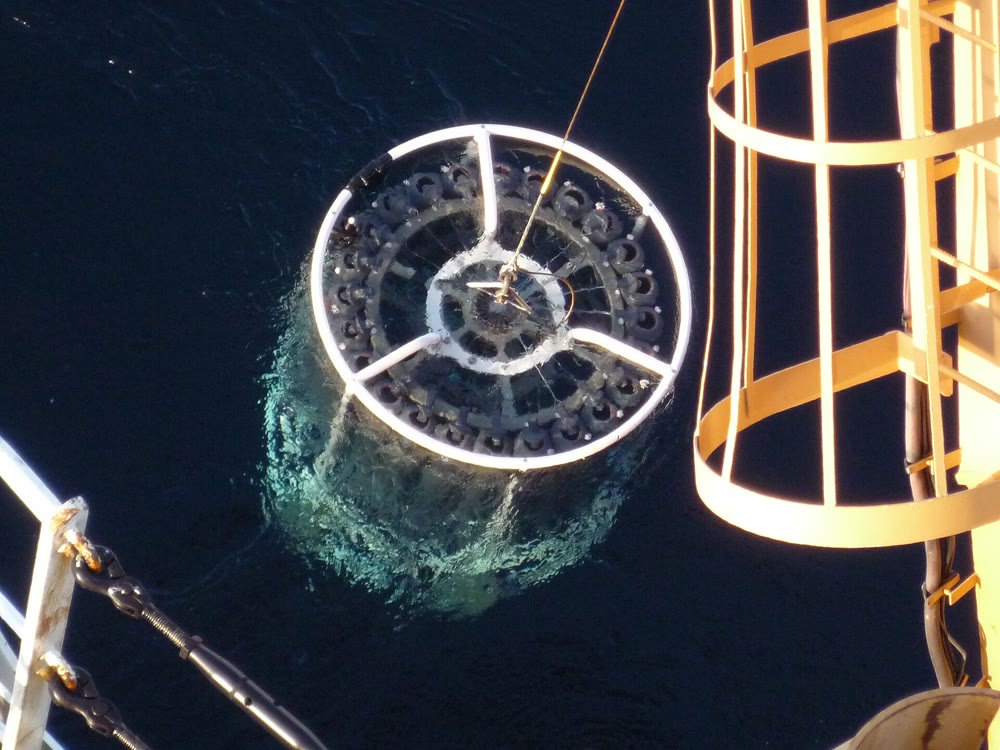
\includegraphics[height=4.4cm]{images/book2/g10-noaa-ctd-rosette.jpg}\hspace{0.4cm}%
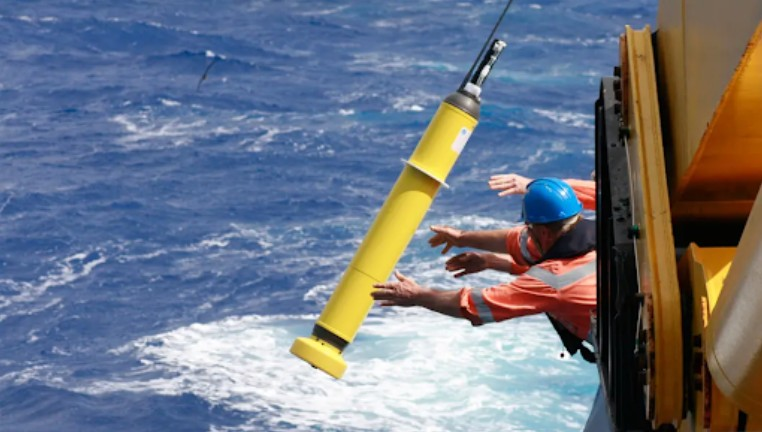
\includegraphics[height=4.4cm]{images/book2/g10-noaa-argo-float.jpg}

{\small Kiri: roset botol sampel di sekeliling sensor-sensornya, ditarik
kembali ke atas di samping kapal riset di Arktika, 2008 (foto: Pablo
Clemente-Colon, NOAA Photo Library). Kanan: sebuah pelampung pemrofil
diluncurkan dari kapal riset (foto: NOAA Global Ocean Monitoring and Observing
Program). Keduanya domain publik.}
\end{omfigure}

Dirata-ratakan atas puluhan tahun pengukuran, profil-profil ini memberikan
gambaran samudra menurut kedalamannya. Profil-profil dalam bab ini adalah
rata-rata seperti itu, dari \emph{World Ocean Atlas 2023} milik NOAA National
Centers for Environmental Information.

\section{Suhu terhadap kedalaman}

\begin{omfigure}
\begin{tikzpicture}
\begin{axis}[omrecord, omdepth, width=0.62\linewidth, height=8.2cm,
  axis x line=top, xmin=-3, xmax=31, ymin=0, ymax=2000,
  xlabel={suhu (\unit{\degreeCelsius})}, ylabel={kedalaman (\unit{m})},
  tick label style={font=\small}, label style={font=\small},
  legend style={font=\scriptsize, at={(0.98,0.03)}, anchor=south east}]
\addplot[omThm!85!black, thick] table[x=t, y=depth] {figdata/out/grade-10-ocean_profiles-site-warmpool.dat};
\addplot[omDef!85!black, thick] table[x=t, y=depth] {figdata/out/grade-10-ocean_profiles-site-atlantic.dat};
\addplot[black!70, thick, dashed] table[x=t, y=depth] {figdata/out/grade-10-ocean_profiles-site-arctic.dat};
\legend{{Pasifik tropis, 5.5\textdegree\ LU}, {Atlantik Utara, 40.5\textdegree\ LU}, {Samudra Arktik, 75.5\textdegree\ LU}}
\node[font=\scriptsize, anchor=west] (ml) at (axis cs:21,430) {lapisan tercampur};
\draw[black!50] (ml.north east) -- (axis cs:28.9,35);
\node[font=\scriptsize, anchor=west] (tc) at (axis cs:15.5,600) {termoklin};
\draw[black!50] (tc.north) -- (axis cs:19.9,150);
\node[font=\scriptsize, anchor=west] at (axis cs:7,1500) {samudra dalam};
\end{axis}
\end{tikzpicture}

{\small Suhu rata-rata terhadap kedalaman di tiga lokasi (kedalaman bertambah
ke bawah). Data: World Ocean Atlas 2023, rata-rata tahunan, NOAA NCEI.}
\end{omfigure}
% ledger: data:b2-woa23 (profiles in figdata/grade-10/ocean_profiles.py)

Cahaya Matahari memanaskan samudra dari atas, di lapisan permukaannya. Angin
dan ombak mengaduk air hangat ini menjadi lapisan yang suhunya hampir seragam.
Di bawahnya, suhu turun dengan cepat sepanjang beberapa ratus meter; lebih
dalam lagi, suhu turun perlahan sampai ke air dingin yang mengisi
cekungan-cekungan samudra.

\begin{definition}[Lapisan tercampur]\label{def:g10:layered-ocean:mixed-layer}
Yang disebut \emph{lapisan tercampur}\index{lapisan tercampur} adalah lapisan
permukaan samudra, yang diaduk oleh angin dan ombak, tempat suhu dan
salinitas hampir tidak berubah terhadap kedalaman.
\end{definition}

\begin{definition}[Termoklin; haloklin; piknoklin; samudra dalam]\label{def:g10:layered-ocean:thermocline}
Yang disebut \emph{termoklin}\index{termoklin} adalah lapisan di bawah \omterm{def:g10:layered-ocean:mixed-layer}{lapisan
tercampur} tempat suhu turun dengan cepat terhadap kedalaman. Lapisan tempat
salinitas berubah dengan cepat terhadap kedalaman disebut
\emph{haloklin}\index{haloklin}; lapisan tempat massa jenis bertambah dengan
cepat terhadap kedalaman disebut \emph{piknoklin}\index{piknoklin}. Di
bawahnya terletak \emph{samudra dalam}\index{samudra dalam}, yang dingin dan
berubah perlahan.
\end{definition}

Di Pasifik tropis \omterm{def:g10:layered-ocean:mixed-layer}{lapisan tercampur} bersuhu \qty{29.2}{\degreeCelsius} dan
tebalnya sekitar \qty{60}{m}; di antara \qty{70}{m} dan \qty{300}{m} suhu
turun hampir sembilan belas derajat, dan pada \qty{1000}{m} suhu tinggal
\qty{4.5}{\degreeCelsius}. Di Atlantik Utara permukaannya lebih sejuk dan
penurunannya lebih bertahap. Di Samudra Arktik seluruh kolom air tetap dalam
rentang dua derajat dari \qty{0}{\degreeCelsius}: hampir tidak ada lapisan
permukaan yang hangat.
% ledger: data:b2-woa23

\begin{method}[Membaca profil samudra]\label{met:g10:layered-ocean:profile}
\begin{enumerate}
  \item Kenali sumbu-sumbunya: kedalaman bertambah ke bawah, besaran yang
        diukur dibaca di sepanjang bagian atas.
  \item \omterm{def:g10:layered-ocean:mixed-layer}{Lapisan tercampur} adalah bagian atas tempat kurva hampir tegak;
        kedalamannya adalah tempat kurva mulai membelok (aturan yang umum:
        tempat suhu telah turun \qty{0.5}{\degreeCelsius} di bawah nilai
        permukaannya).
  \item \omterm{def:g10:layered-ocean:thermocline}{Termoklin} adalah tempat kurva paling mendekati mendatar: perubahan
        terbesar untuk kedalaman terkecil.
  \item Di bawahnya, bacalah nilai-nilai dalam dan bandingkan lokasi-lokasi
        pada kedalaman yang sama.
\end{enumerate}
\end{method}

\omterm{def:g10:layered-ocean:mixed-layer}{Lapisan tercampur} berubah menurut musim. Pada musim dingin permukaan
kehilangan kalor, badai mengaduk laut, dan \omterm{def:g10:layered-ocean:mixed-layer}{lapisan tercampur} menjadi lebih
dalam; pada musim panas Matahari menghangatkan lapisan permukaan yang tipis
yang tidak dapat dicampur ke bawah oleh angin yang lebih lemah, dan sebuah
\emph{\omterm{def:g10:layered-ocean:thermocline}{termoklin} musiman} terbentuk di dekat permukaan --- air dingin yang
ditemukan oleh kaki si perenang.

\begin{omfigure}
\begin{tikzpicture}
\begin{axis}[omrecord, omdepth, width=0.6\linewidth, height=6.6cm,
  axis x line=top, xmin=12, xmax=24, ymin=0, ymax=300,
  xlabel={suhu (\unit{\degreeCelsius})}, ylabel={kedalaman (\unit{m})},
  tick label style={font=\small}, label style={font=\small},
  legend style={font=\scriptsize, at={(0.98,0.03)}, anchor=south east}]
\addplot[omDef!85!black, thick] table[x=t_feb, y=depth] {figdata/out/grade-10-ocean_profiles-season.dat};
\addplot[omThm!85!black, thick] table[x=t_aug, y=depth] {figdata/out/grade-10-ocean_profiles-season.dat};
\legend{Februari, Agustus}
\end{axis}
\end{tikzpicture}

{\small Musim dingin dan musim panas di Atlantik Utara (40.5\textdegree\ LU,
30.5\textdegree\ BB): suhu rata-rata bulanan untuk Februari dan Agustus. Pada
bulan Februari \omterm{def:g10:layered-ocean:mixed-layer}{lapisan tercampur} mencapai sekitar \qty{170}{m}; pada bulan
Agustus lapisan hangat setebal sekitar \qty{15}{m} terletak di atas \omterm{def:g10:layered-ocean:thermocline}{termoklin}
musiman. Data: World Ocean Atlas 2023, NOAA NCEI.}
\end{omfigure}
% ledger: data:b2-woa23 (mixed-layer depths by the 0.5 degC rule, computed in figdata/grade-10/ocean_profiles.py)

\section{Salinitas dan massa jenis}

Massa jenis air laut bergantung pada suhu dan salinitasnya. Massa jenis itu
dihitung dengan rumus yang disepakati secara internasional, yaitu persamaan
keadaan air laut, yang dicocokkan dengan pengukuran laboratorium.

\begin{proposition}[Massa jenis air laut]\label{prop:g10:layered-ocean:density}
Massa jenis air laut bertambah dengan salinitasnya dan berkurang ketika suhunya
naik. Pada tekanan permukaan, air laut bersalinitas 35 memiliki massa jenis
\qty{1028.1}{kg/m^3} pada \qty{0}{\degreeCelsius} dan \qty{1023.3}{kg/m^3}
pada \qty{25}{\degreeCelsius}; air murni pada \qty{4}{\degreeCelsius} memiliki
massa jenis \qty{1000.0}{kg/m^3}.
\end{proposition}
% ledger: unesco:eos80 (values computed in figdata/grade-10/ocean_profiles.py)

\begin{omfigure}
\begin{tikzpicture}
\begin{axis}[omrecord, width=0.7\linewidth, height=6.2cm, xmin=-2, xmax=30,
  ymin=1016, ymax=1033, xlabel={suhu (\unit{\degreeCelsius})},
  ylabel={massa jenis (\unit{kg/m^3})}, tick label style={font=\small},
  label style={font=\small}, yticklabel style={/pgf/number format/1000 sep={}}]
\addplot[omThm!85!black, thick] table[x=t, y=rho_s38] {figdata/out/grade-10-ocean_profiles-eos.dat};
\addplot[black!80, thick] table[x=t, y=rho_s35] {figdata/out/grade-10-ocean_profiles-eos.dat};
\addplot[omDef!85!black, thick] table[x=t, y=rho_s30] {figdata/out/grade-10-ocean_profiles-eos.dat};
\node[font=\scriptsize, anchor=south west, omThm!85!black] at (axis cs:1,1030.75) {salinitas 38};
\node[font=\scriptsize, anchor=south west] at (axis cs:1,1028.35) {salinitas 35};
\node[font=\scriptsize, anchor=south west, omDef!85!black] at (axis cs:1,1024.35) {salinitas 30};
\end{axis}
\end{tikzpicture}

{\small Massa jenis air laut pada tekanan permukaan, terhadap suhunya, untuk
tiga salinitas (dihitung dari persamaan keadaan air laut internasional).}
\end{omfigure}
% ledger: unesco:eos80

Dua hal terlihat pada grafik itu. Satu satuan salinitas menambah sekitar
\qty{0.8}{kg/m^3}. Pemanasan satu derajat mengurangi sekitar
\qty{0.31}{kg/m^3} pada \qty{25}{\degreeCelsius}, \qty{0.18}{kg/m^3} pada
\qty{10}{\degreeCelsius}, tetapi hanya \qty{0.06}{kg/m^3} di dekat
\qty{0}{\degreeCelsius}: di laut yang hangat suhulah yang mengendalikan massa
jenis, di laut yang dingin salinitaslah yang mengendalikannya.
% ledger: unesco:eos80 (slopes computed in figdata/grade-10/ocean_profiles.py)

\begin{remark}
Massa jenis dalam bab ini dihitung pada tekanan permukaan. Tekanan air di
atasnya sedikit memampatkan air laut, sekitar \qty{4}{kg/m^3} per kilometer
kedalaman; para oseanograf membandingkan massa-massa air pada tekanan yang
sama, sehingga hanya suhu dan salinitas yang berpengaruh.
\end{remark}
% ledger: unesco:eos80-checks (computed in figdata/grade-10/ocean_profiles.py: 3.9 kg/m3 per km from the 10000-dbar check values)

\begin{omfigure}
\begin{tikzpicture}
\begin{axis}[name=sal, omrecord, omdepth, width=0.5\linewidth, height=7.2cm,
  axis x line=top, xmin=27.5, xmax=37, ymin=0, ymax=1000,
  xlabel={salinitas}, ylabel={kedalaman (\unit{m})},
  tick label style={font=\small}, label style={font=\small}]
\addplot[omThm!85!black, thick] table[x=s, y=depth] {figdata/out/grade-10-ocean_profiles-site-warmpool.dat};
\addplot[omDef!85!black, thick] table[x=s, y=depth] {figdata/out/grade-10-ocean_profiles-site-atlantic.dat};
\addplot[black!70, thick, dashed] table[x=s, y=depth] {figdata/out/grade-10-ocean_profiles-site-arctic.dat};
\node[font=\scriptsize, anchor=west, align=left] at (axis cs:28.2,120) {haloklin\\Arktik};
\end{axis}
\begin{axis}[at={(sal.east)}, anchor=west, xshift=0.9cm, omrecord, omdepth,
  width=0.5\linewidth, height=7.2cm, axis x line=top, xmin=1021, xmax=1028.5, yticklabels={},
  ymin=0, ymax=1000, xlabel={massa jenis (\unit{kg/m^3})},
  tick label style={font=\small}, label style={font=\small},
  xticklabel style={/pgf/number format/1000 sep={}},
  legend style={font=\scriptsize, at={(0.03,0.03)}, anchor=south west}]
\addplot[omThm!85!black, thick] table[x=rho, y=depth] {figdata/out/grade-10-ocean_profiles-site-warmpool.dat};
\addplot[omDef!85!black, thick] table[x=rho, y=depth] {figdata/out/grade-10-ocean_profiles-site-atlantic.dat};
\addplot[black!70, thick, dashed] table[x=rho, y=depth] {figdata/out/grade-10-ocean_profiles-site-arctic.dat};
\legend{Pasifik tropis, Atlantik Utara, Samudra Arktik}
\end{axis}
\end{tikzpicture}

{\small Salinitas (kiri) dan massa jenis pada tekanan permukaan (kanan)
terhadap kedalaman, di tiga lokasi profil suhu. Di setiap lokasi massa jenis
bertambah ke arah bawah. Data: World Ocean Atlas 2023, NOAA NCEI; massa jenis
dari persamaan keadaan air laut internasional.}
\end{omfigure}
% ledger: data:b2-woa23, unesco:eos80

Di Pasifik tropis \omterm{def:g10:layered-ocean:thermocline}{piknoklin} berimpit dengan \omterm{def:g10:layered-ocean:thermocline}{termoklin}. Di Samudra Arktik suhu
hampir tidak berubah, tetapi salinitas naik dari 28 di permukaan, yang
ditawarkan oleh sungai-sungai dan es yang mencair, menjadi 34.8 pada
\qty{500}{m}: \omterm{def:g10:layered-ocean:thermocline}{haloklin} adalah \omterm{def:g10:layered-ocean:thermocline}{piknoklinnya}. Dalam setiap kasus massa jenis
bertambah ke arah bawah.
% ledger: data:b2-woa23

\begin{definition}[Stratifikasi]\label{def:g10:layered-ocean:stratification}
Samudra disebut \emph{terstratifikasi}\index{stratifikasi} bila massa jenisnya
bertambah terhadap kedalaman: air yang lebih ringan terletak di atas air yang
lebih rapat, berlapis-lapis.
\end{definition}

Samudra yang \omterm{def:g10:layered-ocean:stratification}{terstratifikasi} bersifat stabil. Sebuah parsel air yang didorong
ke bawah ke dalam air yang lebih rapat lebih ringan daripada sekitarnya dan
mengapung naik kembali; parsel yang didorong ke atas tenggelam kembali. Untuk
mencampur lapisan-lapisan itu, angin harus bekerja melawan hal ini, dan makin
kuat \omterm{def:g10:layered-ocean:thermocline}{piknoklinnya}, makin sulit pencampurannya: \omterm{def:g10:layered-ocean:thermocline}{termoklin} adalah tutup yang
memisahkan permukaan dari \omterm{def:g10:layered-ocean:thermocline}{samudra dalam}. \omterm{def:g10:layered-ocean:thermocline}{Samudra dalam} diisi oleh air yang
dahulu kala tenggelam dari laut-laut kutub yang dingin, tempat air permukaan
menjadi cukup rapat untuk tenggelam (Buku 1, kelas 8).

\section{Penaikan massa air}

\begin{definition}[Penaikan massa air]\label{def:g10:layered-ocean:upwelling}
Yang disebut \emph{penaikan massa air}\index{penaikan massa air} adalah
naiknya air dingin dari bawah lapisan permukaan untuk menggantikan air
permukaan yang didorong menjauh oleh angin. Penaikan massa air terjadi di
sepanjang beberapa pesisir dan di samudra terbuka.
\end{definition}
% ledger: noaa:upwelling

Di sepanjang pesisir, angin yang bertiup sejajar dengan garis pantai menyeret
air permukaan; karena rotasi Bumi, air itu tidak sekadar mengikuti angin
tetapi dibelokkan darinya, ke kanan di belahan bumi utara dan ke kiri di
belahan bumi selatan (cara kerjanya dibahas dalam jilid-jilid universitas). Di
lepas pantai Peru angin bertiup di sepanjang pantai ke arah khatulistiwa, dan
air permukaan didorong ke laut lepas; air dingin naik di dekat pesisir untuk
menggantikannya. \omterm{def:g10:layered-ocean:upwelling}{Penaikan massa air} juga terjadi di sepanjang khatulistiwa,
tempat angin pasat mendorong air permukaan menjauhinya di kedua sisi.
% ledger: noaa:upwelling, kessler:peru-upwelling

\begin{omfigure}
\begin{tikzpicture}[font=\footnotesize, >={Stealth[length=2mm]}]
  % ocean and thermocline
  \fill[omDef!12] (0,-3.2) rectangle (8.2,0);
  \fill[omDef!30] (0,-3.2) -- (0,-2.0) .. controls (3,-2.0) and (5.5,-1.6) .. (7.4,-0.35) -- (8.2,0) -- (8.2,-3.2) -- cycle;
  \draw[omDef!80!black, dashed] (0,-2.0) .. controls (3,-2.0) and (5.5,-1.6) .. (7.4,-0.35);
  \node[anchor=north west, omDef!80!black] at (0.1,-2.05) {termoklin};
  \node[anchor=west, black!70] at (0.15,-0.9) {air permukaan yang hangat};
  \node[anchor=west, black!70] at (0.15,-2.75) {air dingin yang kaya nutrien};
  % land
  \fill[omExo!30, draw=black!60] (7.0,-3.2) -- (8.2,-0.1) -- (8.6,0.0) -- (9.6,1.2) -- (10.6,2.2) -- (10.6,-3.2) -- cycle;
  \node[anchor=south, align=center] at (9.9,-1.6) {daratan};
  % surface flow and rising water
  \draw[->, thick, omThm!80!black] (7.2,-0.3) -- (3.6,-0.3);
  \node[anchor=south, omThm!80!black] at (5.4,-0.25) {air permukaan didorong ke laut lepas};
  \foreach \x/\y in {6.1/-2.1, 6.8/-1.7} \draw[->, thick, omDef!80!black] (\x,\y) -- (\x+0.45,\y+1.15);
  \node[anchor=north, omDef!80!black, align=center] at (6.0,-2.25) {air dingin naik};
  % wind along the shore, northward: with west on the left and east on the
  % right the reader looks north, so the wind goes into the page
  \draw[black!70, thick] (2.6,1.0) circle (0.22);
  \draw[black!70, thick] (2.6,1.0) ++(45:0.22) -- ++(225:0.44) (2.6,1.0) ++(135:0.22) -- ++(315:0.44);
  \node[anchor=west, align=left] at (2.9,1.0) {angin di sepanjang pantai, ke arah khatulistiwa\\(ke utara, masuk ke halaman)};
  \node[anchor=north west, black!60] at (0,-3.25) {$\leftarrow$ barat};
  \node[anchor=north east, black!60] at (10.6,-3.25) {timur $\rightarrow$};
\end{tikzpicture}

{\small \omterm{def:g10:layered-ocean:upwelling}{Penaikan massa air} pesisir di lepas pantai Peru (penampang skematis
dari barat ke timur, tidak berskala): angin bertiup di sepanjang pantai ke
arah khatulistiwa, ke utara, masuk ke halaman; air permukaan dibelokkan ke
kirinya dan didorong ke laut lepas; air dingin dari bawah \omterm{def:g10:layered-ocean:thermocline}{termoklin} naik di
dekat pesisir untuk menggantikannya.}
\end{omfigure}

Air yang naik itu tidak hanya dingin. Di bawah lapisan permukaan yang
tersinari Matahari, sisa-sisa plankton mati yang tenggelam dan membusuk
melepaskan nutrien mineral yang diperlukan fitoplankton. Setelah dibawa
kembali ke dalam cahaya, nutrien ini menjadikan daerah-daerah \omterm{def:g10:layered-ocean:upwelling}{penaikan massa
air} perairan yang paling produktif di samudra, dengan daerah penangkapan ikan
yang paling kaya. Di tempat samudra \omterm{def:g10:layered-ocean:stratification}{terstratifikasi} dengan kuat dan tidak ada
yang membawa air dalam ke atas, lapisan yang tersinari Matahari kehabisan
nutrien: pusat-pusat pilin subtropis adalah gurun-gurun samudra.
% ledger: noaa:upwelling

\begin{omfigure}
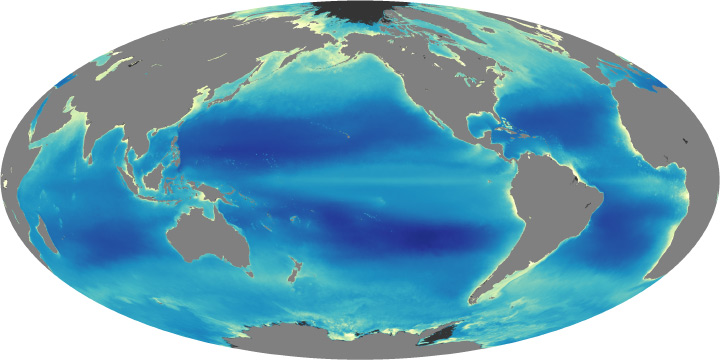
\includegraphics[width=0.8\linewidth]{images/book2/g10-nasa-ocean-chlorophyll.jpg}

{\small Klorofil fitoplankton dilihat dari angkasa, dirata-ratakan atas
2002--2010: dari biru tua (sangat sedikit) melalui biru muda sampai kuning
(banyak); daratan berwarna kelabu. Pesisir Peru dan pita di sepanjang
khatulistiwa di Pasifik tampak menonjol; pilin-pilinnya berwarna biru tua.
Citra: Jesse Allen dan Robert Simmon, NASA Earth Observatory (domain publik).}
\end{omfigure}

\begin{omfigure}
\begin{tikzpicture}
\begin{axis}[omrecord, omdepth, width=0.6\linewidth, height=7.2cm,
  axis x line=top, xmin=4, xmax=26, ymin=0, ymax=600,
  xlabel={suhu (\unit{\degreeCelsius})}, ylabel={kedalaman (\unit{m})},
  tick label style={font=\small}, label style={font=\small},
  legend style={font=\scriptsize, at={(0.98,0.03)}, anchor=south east}]
\addplot[omExo!85!black, thick] table[x=t, y=depth] {figdata/out/grade-10-ocean_profiles-site-peru.dat};
\addplot[omThm!85!black, thick] table[x=t, y=depth] {figdata/out/grade-10-ocean_profiles-site-gyre.dat};
\addplot[black!40, dashed, domain=0:600, samples=2] ({15}, {x});
\legend{{lepas pantai Peru, 13.5\textdegree\ LS}, {pilin Pasifik Selatan, 20.5\textdegree\ LS}}
\end{axis}
\end{tikzpicture}

{\small Di lepas pantai Peru, air dingin mendekati permukaan: air bersuhu
\qty{15}{\degreeCelsius} (garis putus-putus) terletak pada sekitar
\qty{65}{m}, dibandingkan dengan hampir \qty{300}{m} di tengah pilin Pasifik
Selatan, yang lebih jauh dari khatulistiwa. Data: World Ocean Atlas 2023,
rata-rata tahunan, NOAA NCEI.}
\end{omfigure}
% ledger: data:b2-woa23

\section{Latihan}

\begin{exercise}[$\star$]\label{exo:g10:layered-ocean:1}
Definisikan \omterm{def:g10:layered-ocean:mixed-layer}{lapisan tercampur} dan \omterm{def:g10:layered-ocean:thermocline}{termoklin}. Apa yang mengaduk \omterm{def:g10:layered-ocean:mixed-layer}{lapisan tercampur}?
\end{exercise}

\begin{exercise}[$\star$]\label{exo:g10:layered-ocean:2}
Definisikan \omterm{def:g10:layered-ocean:upwelling}{penaikan massa air}. Mengapa perairan di daerah \omterm{def:g10:layered-ocean:upwelling}{penaikan massa air} kaya akan kehidupan?
\end{exercise}

\begin{exercise}[$\star$]\label{exo:g10:layered-ocean:3}
Dengan profil suhu ketiga lokasi, sebutkan suhu di permukaan dan pada
\qty{1000}{m} di Pasifik tropis dan di Samudra Arktik.
\end{exercise}

\begin{exercise}[$\star$]\label{exo:g10:layered-ocean:4}
Manakah yang lebih rapat, air laut bersalinitas 35 pada
\qty{25}{\degreeCelsius} atau pada \qty{0}{\degreeCelsius}? Air laut
bersalinitas 35 atau air murni, pada suhu yang sama? Gunakan nilai-nilai dalam
bab ini.
\end{exercise}

\begin{exercise}[$\star$]\label{exo:g10:layered-ocean:5}
Jelaskan bagaimana pelampung pemrofil mengukur profil samudra, dan mengapa
pelampung berguna di tempat yang jarang didatangi kapal.
\end{exercise}

\begin{exercise}[$\star\star$]\label{exo:g10:layered-ocean:6}
Samudra meliputi \num{361.84}~juta~\unit{km^2} dengan kedalaman rata-rata
\qty{3682}{m}. Hitung volumenya dalam kilometer kubik. Berapa bagian dari
kedalamannya yang diwakili oleh \qty{100}{m} teratas?
\end{exercise}

\begin{exercise}[$\star\star$]\label{exo:g10:layered-ocean:7}
Pada profil Atlantik Utara bulan Agustus, suhu adalah
\qty{22.7}{\degreeCelsius} di permukaan, \qty{22.2}{\degreeCelsius} pada
\qty{15}{m}, \qty{21.8}{\degreeCelsius} pada \qty{20}{m}, dan
\qty{17.3}{\degreeCelsius} pada \qty{50}{m}. Dengan aturan dalam metode,
perkirakan kedalaman \omterm{def:g10:layered-ocean:mixed-layer}{lapisan tercampur}. Berapa laju rata-rata penurunan suhu
di antara \qty{20}{m} dan \qty{50}{m}, dalam derajat per meter?
\end{exercise}

\begin{exercise}[$\star\star$]\label{exo:g10:layered-ocean:8}
Di lokasi Atlantik Utara yang sama, permukaan bersuhu \qty{15.3}{\degreeCelsius}
pada bulan Februari dan \qty{22.7}{\degreeCelsius} pada bulan Agustus,
sedangkan pada \qty{300}{m} suhunya \qty{13.5}{\degreeCelsius} pada kedua
bulan itu. Jelaskan mengapa air dalam tidak mengikuti musim, dan mengapa
\omterm{def:g10:layered-ocean:mixed-layer}{lapisan tercampur} musim dingin jauh lebih dalam daripada \omterm{def:g10:layered-ocean:mixed-layer}{lapisan tercampur}
musim panas.
\end{exercise}

\begin{exercise}[$\star\star$]\label{exo:g10:layered-ocean:9}
Di dekat \qty{10}{\degreeCelsius}, satu satuan salinitas menambah
\qty{0.78}{kg/m^3} pada massa jenis dan pemanasan satu derajat mengurangi
\qty{0.18}{kg/m^3}. Berapa derajat pemanasan yang meniadakan satu satuan
salinitas? Jawablah pertanyaan yang sama di dekat \qty{0}{\degreeCelsius},
tempat satu derajat hanya mengurangi \qty{0.06}{kg/m^3}. Apa kesimpulanmu
untuk laut-laut kutub?
\end{exercise}

\begin{exercise}[$\star\star$]\label{exo:g10:layered-ocean:10}
Di Samudra Arktik air di permukaan bersuhu \qty{-1.4}{\degreeCelsius} dengan
salinitas 28.1, dan pada \qty{200}{m} bersuhu \qty{-1.4}{\degreeCelsius}
dengan salinitas 33.3. Massa jenisnya \qty{1022.6}{kg/m^3} dan
\qty{1026.8}{kg/m^3}. Apa yang membuat air yang lebih dalam lebih rapat?
Sebutkan nama lapisan di antara keduanya.
\end{exercise}

\begin{exercise}[$\star\star$]\label{exo:g10:layered-ocean:11}
Jelaskan mengapa samudra yang \omterm{def:g10:layered-ocean:stratification}{terstratifikasi} bersifat stabil, dengan memakai
sebuah parsel air permukaan yang didorong ke bawah oleh ombak.
\end{exercise}

\begin{exercise}[$\star\star\star$]\label{exo:g10:layered-ocean:12}
Satu liter air laut bersalinitas 35 pada \qty{0}{\degreeCelsius} dihangatkan
menjadi \qty{25}{\degreeCelsius}. Dengan massa jenis dalam bab ini, hitung
massanya, lalu volumenya yang baru. Berapa besar air itu memuai, dalam
mililiter? Lapisan samudra setebal \qty{700}{m} menghangat dengan perbandingan
yang sama: berapa besar tebalnya bertambah? (Ini sangat melebih-lebihkan
pemanasan samudra yang sebenarnya, dan dipakai di sini hanya untuk
memperlihatkan efeknya.)
\end{exercise}

\begin{exercise}[$\star\star\star$]\label{exo:g10:layered-ocean:13}
Di Pasifik tropis massa jenisnya \qty{1021.6}{kg/m^3} pada \qty{50}{m} dan
\qty{1026.0}{kg/m^3} pada \qty{200}{m}; di Atlantik Utara pada bulan Februari
suhu hampir tidak berubah sepanjang \qty{150}{m} teratas. Di manakah dari
keduanya badai lebih mudah mengaduk air sampai \qty{150}{m}? Jelaskan.
\end{exercise}

\begin{exercise}[$\star\star\star$]\label{exo:g10:layered-ocean:14}
Pada peta klorofil, temukan dua daerah berklorofil tinggi di samudra terbuka
yang jauh dari pesisir mana pun, dan satu daerah luas yang klorofilnya sangat
rendah. Dengan isi bab ini, jelaskan masing-masing.
\end{exercise}

\begin{exercise}[$\star\star\star$]\label{exo:g10:layered-ocean:15}
Misalkan sebuah pelampung tenggelam dari \qty{1000}{m} ke \qty{2000}{m} dalam
enam jam, lalu naik ke permukaan dalam sepuluh jam. Hitung laju tegak
rata-ratanya pada setiap tahap, dalam sentimeter per detik. Jika pelampung itu
mengukur setiap \qty{2}{s} selama naik, berapa banyak pengukuran dalam satu
profil, dan berapa rata-rata jarak kedalaman di antara dua pengukuran?
\end{exercise}

\section{Soal: Sebuah Pengukuran di Lepas Pantai Peru}

\begin{problem}[{Soal akhir pekan --- dua profil Pasifik Selatan}]
\label{pb:g10:layered-ocean:1}
% ledger: data:b2-woa23, unesco:eos80 (values rounded from figdata/grade-10/ocean_profiles.py)
Tabel ini memberikan suhu dan salinitas rata-rata, serta massa jenis yang
dihitung pada tekanan permukaan, di dua tempat di Pasifik Selatan: di lepas
pantai Peru (\qty{13.5}{\degree} LS, \qty{77.5}{\degree} BB) dan di tengah
pilin subtropis (\qty{20.5}{\degree} LS, \qty{110.5}{\degree} BB).

\begin{center}
\small
\begin{tabular}{c|ccc|ccc}
\hline
 & \multicolumn{3}{c|}{lepas pantai Peru} & \multicolumn{3}{c}{pilin} \\
kedalaman (\unit{m}) & \unit{\degreeCelsius} & salinitas & \unit{kg/m^3} & \unit{\degreeCelsius} & salinitas & \unit{kg/m^3} \\
\hline
0 & 19.0 & 35.08 & 1025.08 & 24.0 & 36.41 & 1024.71 \\
25 & 17.4 & 35.06 & 1025.47 & 23.9 & 36.39 & 1024.73 \\
50 & 15.8 & 35.03 & 1025.83 & 23.6 & 36.38 & 1024.80 \\
100 & 13.7 & 34.93 & 1026.20 & 22.6 & 36.27 & 1025.02 \\
200 & 12.4 & 34.89 & 1026.44 & 20.3 & 35.80 & 1025.30 \\
300 & 11.1 & 34.80 & 1026.62 & 14.4 & 34.76 & 1025.92 \\
500 & 7.9 & 34.60 & 1026.97 & 7.1 & 34.39 & 1026.92 \\
\hline
\end{tabular}
\end{center}

\medskip
\noindent\textbf{Bagian I --- Membaca profil.}
\begin{enumerate}
  \item Lokasi manakah yang lebih hangat di permukaan, dan seberapa banyak?
  \item Lokasi manakah yang lebih jauh dari khatulistiwa? Apakah selisih suhu
        permukaan itu sesuai dengan yang kamu harapkan dari lintangnya saja?
  \item Dengan aturan dalam metode, perkirakan kedalaman \omterm{def:g10:layered-ocean:mixed-layer}{lapisan tercampur}
        di pilin.
  \item Apakah ada \omterm{def:g10:layered-ocean:mixed-layer}{lapisan tercampur} di lepas pantai Peru? Uraikan
        \qty{100}{m} teratasnya.
  \item Di antara kedalaman berapa suhu turun paling cepat di pilin?
        Sebutkan lajunya, dalam derajat per seratus meter.
  \item Kira-kira pada kedalaman berapa air bersuhu \qty{15}{\degreeCelsius}
        di setiap lokasi?
\end{enumerate}

\medskip
\noindent\textbf{Bagian II --- Massa jenis.}
\begin{enumerate}[resume]
  \item Periksalah bahwa massa jenis bertambah terhadap kedalaman di kedua
        lokasi. Apa yang diberitahukan hal ini tentang kestabilannya?
  \item Di pilin, air permukaan lebih asin daripada di lepas pantai Peru.
        Apakah hal ini seharusnya membuatnya lebih rapat atau lebih ringan?
        Apakah air itu memang lebih rapat?
  \item Jelaskan efek mana dari keduanya yang menang.
  \item Hitung pertambahan massa jenis dari permukaan sampai \qty{200}{m}
        di lepas pantai Peru.
  \item Hitung pertambahan yang sama di pilin.
\end{enumerate}

\medskip
\noindent\textbf{Bagian III --- Membandingkan stratifikasi.}
\begin{enumerate}[resume]
  \item Di pilin, di manakah sebagian besar pertambahan massa jenis pada
        \qty{500}{m} teratas ditemukan: di atas atau di bawah \qty{200}{m}?
  \item Di lepas pantai Peru, di manakah pertambahan itu ditemukan?
  \item Pada \qty{500}{m}, bandingkan kedua lokasi. Apa yang diisyaratkan hal
        ini tentang air dalam di bawah keduanya?
  \item Jelaskan dalam beberapa kalimat bagaimana \omterm{def:g10:layered-ocean:thermocline}{termoklin} di lepas pantai
        Peru telah terangkat ke arah permukaan.
  \item Fitoplankton hidup di beberapa puluh meter teratas. Di lokasi manakah
        air kaya nutrien dari bawah \omterm{def:g10:layered-ocean:thermocline}{termoklin} berada dalam jangkauan
        pengadukan oleh angin? Jelaskan.
\end{enumerate}

\medskip
\noindent\textbf{Bagian IV --- Mengapa perairan Peru produktif.}
\begin{enumerate}[resume]
  \item Akan seperti apakah air permukaan di lepas pantai Peru jika angin di
        sepanjang pantai berhenti bertiup selama berbulan-bulan?
  \item Dengan peta klorofil, bandingkan kedua lokasi.
  \item Jelaskan mengapa pilin disebut gurun samudra meskipun pilin itu penuh
        cahaya Matahari.
  \item Hitung perbandingan pertambahan massa jenis dari permukaan sampai
        \qty{200}{m} di lepas pantai Peru dan di pilin, lalu jelaskan apa yang
        diperlihatkannya.
\end{enumerate}
\end{problem}
